\documentclass[12pt,a4paper]{scrartcl} 

%Deutsch:
	\usepackage[ngerman]{babel} %Deutsches Datumformat, Umlaute m\"oglich,...
	\usepackage[utf8]{inputenc}
	\usepackage[T1]{fontenc} 
	
%Quellenverzeichnis:
	\usepackage[maxcitenames=2,autocite=footnote,uniquename=full,uniquelist=true,backend=biber]{biblatex} %style=authoryear-icomp
	\usepackage{csquotes} %Hilfspaket für Biblatex
	\bibliography{bib_database.bib} %Datei mit bibliographischen Daten
	\DefineBibliographyStrings{ngerman}{andothers={et\ al\adddot}} % "u.a." zu "et al."
	\DefineBibliographyStrings{ngerman}{and={\&}} % "und" zu "&"

%Mathematik:
	\usepackage{dsfont} %Symbole
	\usepackage{amsmath} %Umgebung
	\usepackage{amssymb} %Symbole
	\usepackage{bbm} %doppelstreifen bei buchstaben (zb symbol für ganze zahlen \mathbbm{Z})
	
%Grafiken:
	\usepackage{graphics}
	\usepackage{graphicx}
	\usepackage{picinpar} %bilder so einfügen, dass text um bilder weiterläuft
	\usepackage{float} %\begin{figure}[H] => Grafik wird HIER eingefügt!

%Euro-Zeichen:
	\usepackage{eurosym}

%Quellcode:
	%\usepackage[numbered,framed]{mcode} %Quellcode darstellen
	
%Englisch:
	%\usepackage[ngerman,english]{babel} %automatisch erzeugte Überschriften etc. auf englisch
	
\DeclareMathOperator*{\argmin}{arg\,min} % Importiere die Einstellungen aus der Präambel

%%%%%%%%%%%%%%%%%%%%%%%%%%%%%%%%%%%%%%%%%%%%%%%%%%%%%%%%%%
% Hier können die Pakete, die benötigten Daten und Graphen für R geladen bzw erstellt werden.
% echo=FALSE gibt keinen R Output wieder
% warum wird der folgende chunk nicht übernommen?



% hier beginnt der eigentliche Inhalt
\usepackage{Sweave}
\begin{document}
\Sconcordance{concordance:Bericht_Sweave.tex:Bericht_Sweave.Rnw:%
1 15 1 1 7 5 1 1 0 28 1 2 2 7 1}


% Deckblatt
\begin{titlepage}
	\rmfamily
	\begin{center}
		% Logo
		%\includegraphics[width=0.15\textwidth]{./logo}\\[1cm]
	
		\textsc{\LARGE Statistisches Consulting}\\[1.5cm]

		\textsc{
			\large{	Master Studiengang Statistik\\[0.25cm]
							Institut für Statistik\\[0.25cm]
							Ludwig-Maximilians-Universität München}}\\[0.25cm]
						
		% Title
		\newcommand{\HRule}{\rule{\linewidth}{0.5mm}}
		\HRule \\[0.4cm]
		{\huge \bfseries Online-Marketing der Interhyp AG\\[0.5cm]Analyse von Tracking-Daten}\\[0.4cm]
		\HRule \\[1.5cm]
		
		% Autoren
		\textbf{Daniel Fuckner} d.fuckner@gmx.de\\
		\textbf{Markus Vogler} markus@vogler-lindau.de\\[1.5cm]
	
		% Betreuer und Projektpartner
		\begin{minipage}{0.4\textwidth}
			\begin{flushleft}
				Projektpartner:\\
				\textbf{Interhyp AG}
			\end{flushleft}
		\end{minipage}
		\hfill
		\begin{minipage}{0.4\textwidth}
			\begin{flushright}
				Betreuer:\\
				\textbf{Dr. Fabian Scheipl}
			\end{flushright}
		\end{minipage}
		
		\vfill

		% Datum
		{\large München, 11.11.2011}
		
	\end{center}
\end{titlepage}

%\thispagestyle{plain}
\pagenumbering{roman} %römische Seitennummerierung

%Abstract
\begin{abstract}
  \noindent
	\paragraph{Abstract:}
	\paragraph{Background:} In patients with
\end{abstract}

%Inhaltsverzeichnis
\newpage
\tableofcontents

\newpage
\pagenumbering{arabic} %ab hier wieder normale Seitennummerierung

% Hier beginnt der eigentliche Text
\section{Einleitung}

Die Interhyp AG ist Vermittler für private Baufinanzierungen. Das heißt, sie wählt aus einem Angebot von verschiedenen Darlehensgebern die optimale Finanzierungsstruktur für einen Kunden aus. Das Unternehmen wurde 1999 von den ehemaligen Goldman-Sachs-Bankern Robert Haselsteiner und Marcus Wolsdorf gegründet. Sechs Jahre später eröffnete die Interhyp AG erste Niederlassungen und konnte gleichzeitig den erfolgreichsten deutschen Börsengang des Jahres verzeichnen. Nach weiteren drei Jahren erfolgte die Übernahme durch ING DIRECT, der weltweilt größten und erfolgreichsten Direktbanken-Gruppe. Heute ist die Interhyp AG der größte Vermittler für private Baufinanzierungen in Deutschland, wurde acht mal in Folge als "Bester Baufinananzierer" (Zeitschrift \euro, Ausgabe 08/2013) ausgezeichnet und verfügt über mehr als 60 Beratungsstandorte mit über 1.000 Mitarbeitern.\\
Das primäre Ziel des Marketing der Interhyp AG ist die Kundenakquise. Da etwa 80\% aller Kundenanträge online abgeschickt werden, liegt der Fokus der Marketing-Abteilung auf dem Online-Marketing, das über verschiedene Kanäle verfügt. Beispiele sind Kooperationen mit anderen Unternehmen wie Immobilienscout24, bezahlte Anzeigen bei Suchmaschinen, Newsletter oder diverse Bannerschaltungen. Durch Online-Tracking können die Werbekontakte eines potentiellen Kunden mit der Interhyp AG zusammengefasst werden. So entsteht ein sogenannter Funnel, wie es in Abbildung \ref{customerJourney} skizziert ist. Jeder potentielle Kunde hat einen oder mehrere aufeinanderfolgende Kontaktpunkte, wobei jeder Kontaktpunkt die genaue Zeit des Kontaktes sowie die Art des Kontaktes, das heißt die Information über welche Kampagne es zu dem Kontakt kam, enthält. Am Ende eines jeden Funnels steht der Abbruch der Beobachtung oder im Idealfall das Ausfüllen eines Onlineantrages durch den Kunden.
\begin{figure}[H]
    \centering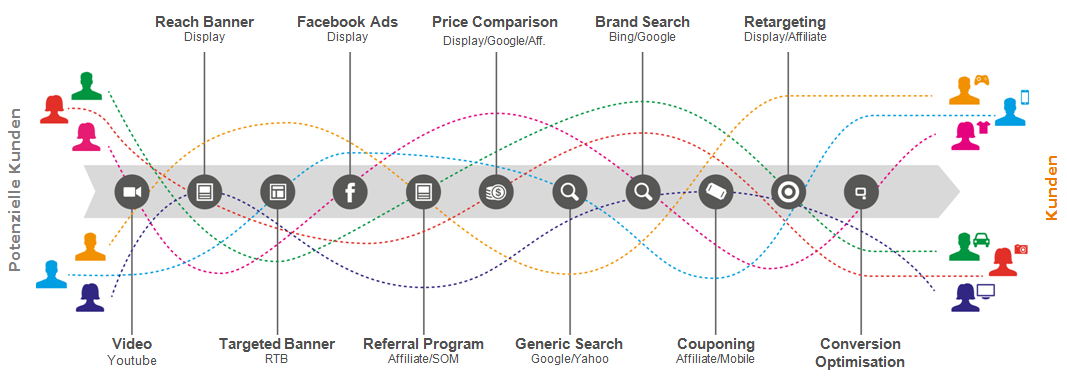
\includegraphics[scale=0.5]{customerJourney.png}\caption[Entstehung eines Funnels]{Entstehung eines Funnels (Quelle: Interhyp AG)}\label{customerJourney}
\end{figure}
\noindent Die Refined Labs GmbH ist auf dem Gebiet des Online-Marketing spezialisiert und verantwortlich für das Online-Tracking der Werbekampagnen der Interhyp AG. Ein Funnel beginnt mit dem ersten Online-Werbekontakt eines potentiellen Kunden mit der Interhyp AG und der damit einhergehenden Erstellung eines Cookies. So können alle weiteren Werbekontakte dem potentiellen Kunden eindeutig zugewiesen werden. Das Tracking endet sobald der potentielle Kunde einen Onlineantrag versendet und damit zum Kunden wird. In diesem Fall spricht man von einem konvertierten Funnel. Wird innerhalb von $90$ Tagen kein Onlineantrag versendet, so wird das Cookie nicht weiter verfolgt und der Funnel wird als nicht-konvertiert bezeichnet.\\
Primäres Ziel dieses Projektes ist das Entdecken von Unterschieden zwischen konvertierten und nicht-konvertierten Funnels. Um dieser Fragestellung gerecht zu werden, wurde ein zeitdiskretes Survival-Modell mittels Stochastic Gradient Boosting geschätzt und ein Sequential Pattern Mining-Algorithmus angewendet. Außerdem wurden die Funnels anhand eines Netzwerkes visualisiert.\\
Die Arbeit ist wie folgt gegliedert. In Kapitel \ref{datenlage} und \ref{descriptiv} werden die Datenaufbereitung und die Variablen erklärt. Daraufhin wird die Methodik des Survival-Modells in Kapitel \ref{survival}, der Sequential Pattern Mining-Algorithmus in Kapitel \ref{spm} und das Netzwerk in Kapitel \ref{network} erläutert. Die Ergebnisse dieser Methoden werden in Kapitel \ref{ergebnisse} vorgestellt und abschließend erfolgt eine Zusammenfassung in Kapitel \ref{zusammenfassung} und die Beschreibung des elektronischen Anhangs in Kapitel \ref{anhang}. % Importiere die Einleitung
\section{Datenlage}\label{datenlage}
%\begin{table}[H]
 %   \begin{center}
  %      \begin{tabular}{|c|p{10cm}|}
   %         \hline $ touchpoint $  & Kontaktpunkt einer Beobachtung \\
    %        \hline $ funnel $ & zeitliche Abfolge der Touchpoints einer Beobachtung\\ 
     %       \hline $ campaign $ & Kategorie der Werbeform auf der obersten Ebene, gegebenfalls auch Ebenen darunter \\ 
      %      \hline $ position \in \{1,2,\dots\}$  & Nummer des Touchpoints eines Funnels\\
       %     \hline $ transaction \in \{0,1\}$  & $1$ steht für konvertiert und $0$ für nicht-konvertiert\\
        %    \hline $ funnelLength \in \{1,2,\dots\} $  & Anzahl der Touchpoints eines Funnels\\
         %   \hline
        %\end{tabular} 
    %\end{center}
    %\caption{Definition der wichtigsten Begriffe}
%\end{table}
Die Daten wurden von der Refined Labs GmbH als SQL-Dump bereitgestellt, der eine Größe von circa $13$ Gigabyte hat. Die MySQL-Datenbank enthält die vier Tabellen \textit{project\_out}, \textit{redirects\_short}, \textit{searchFunnel} und \textit{stage2\_transactionHandling}. Mit Hilfe der vorhanden Informationen in \textit{searchFunnel} und \textit{stage2\_transactionHandling} konnten die Kontaktpunkte in \textit{redirects\_short} in konvertierte und nicht-konvertierte Funnels unterteilt werden. In \textit{projects\_out} sind die Kampagnen in Form einer Baumstruktur organisiert. In Absprache mit der Interhyp AG wurden $17$ Kategorien ausgewählt, die sich auf den ersten drei Ebenen dieser Baumstruktur befinden. Anhand von IDs wurde jedem Kontaktpunkt eine dieser Kategorien zugewiesen.\\
Tabelle \ref{exdata} enthält ein Datenbeispiel mit den Spalten \textit{ID}, \textit{Campaign}, \textit{Transaction}, \textit{First} und \textit{Last}. Das Beispiel enthält zwei verschiedene \textit{IDs}, das heißt zwei Funnels, wobei der erste vier und der zweite drei Kontaktpunkte hat. Die Spalte \textit{Campaign} enthält die Kampagne der Kontaktpunkte. \textit{Transaction}, \textit{First} und \textit{Last} sind binäre Variablen. \textit{Transaction} gibt an, ob der Kunde konvertiert ist, wobei der Wert $1$ nur für den letzten Kontaktpunkt vor der Konvertiertung angenommen wird. Das heißt bei \textit{ID} $1$ handelt es sich um einen konvertierten und bei \textit{ID} $2$ um einen nicht-konvertierten Funnel. \textit{First} beziehungsweise \textit{Last} nimmt den Wert $1$ an, wenn es sich um den ersten beziehungsweise letzten Kontaktpunkt eines Funnels handelt. Die $17$ Kampagnen und weitere Features, die aus den Daten erzeugt wurden, werden in Kapitel \ref{descriptiv} näher erläutert.\\
\begin{table}[H]
	\begin{center}
		\begin{tabular}{|c|l|c|c|c|c|}
			\hline
			ID & Campaign 									 & Transaction & First & Last & ... \\ \hline\hline
			1  & Affiliate - Partnerprogramm & 0					 & 1		 & 0    & ... \\ \hline
			1  & SEM - Brand                 & 0					 & 0		 & 0    & ... \\ \hline
			1  & Direct                      & 0					 & 0		 & 0    & ... \\ \hline
			1  & Direct                      & 1					 & 0		 & 1    & ... \\ \hline
			2  & Display                     & 0					 & 1		 & 0    & ... \\ \hline
			2  & SEM - Generisch             & 0					 & 0		 & 0    & ... \\ \hline
			2  & Social Media                & 0					 & 0		 & 1    & ... \\ \hline
		\end{tabular} 
	\end{center}
	\caption{Beispiel für einen Auszug aus der Datenbank}\label{exdata}
\end{table}
Ein Kontaktpunkt ist entweder ein \textit{Click} oder ein \textit{View}. Man spricht von einem \textit{Click}, wenn der potentielle Kunde tatsächlich etwas angeklickt hat, wobei die genaue Definition von der Kampagne abhängt. Ein \textit{View} wird getrackt, wenn ein Banner oder ähnliches lediglich gesehen, aber nicht angeklickt wird. An dieser Stelle wirft die Datenerhebung allerdings ein Problem für die statistischen Analysen auf. Die \textit{Views} werden für alle konvertierten Funnels gespeichert, für die nicht-konvertierten Funnels allerdings nur, wenn diese bei einem anderen Kunden der Refined Labs GmbH konvertieren. Dass heißt, es ist eine systematische Veränderung der Daten gegeben. Deshalb besteht keine Möglichkeit die \textit{Views} in statistische Analysen, die konvertierte und nicht-konvertierte Funnels vergleichen, einzubeziehen. Die \textit{Views} werden lediglich in Kapitel \ref{descriptiv} in einigen Plots betrachtet, die nur konvertierte Funnels enthalten, und von den weiteren Analysen ausgeschlossen.\\
Nach der Vorverarbeitung der Daten liegen ??? konvertierte und ??? nicht-konvertierte Funnels vor, die nur \textit{Clicks} enthalten. Eine nähere Beschreibung der erstellten Features erfolgt in Kapitel \ref{descriptiv}.




\section{Zeitdiskretes Survival-Modell}\label{survival}

\subsection{Lebensdauer-Modell}\label{secModel1}

Aufgrund der in Kapitel \ref{datenlage} beschriebenen Datenlage erscheint die Anwendung eines Modells aus dem Feld der Lebensdaueranalyse intuitiv. Es wird die Zeit bis zu einem Ereignis betrachtet, welches in diesem Fall das Ausfüllen eines Online-Antrages ist. Der Kunde befindet sich während der Beobachtungsspanne im transienten Zustand bis er durch die Konvertierung in den absorbierenden Zustand wechselt, an dem die Beobachtung endet. Tritt am Ende der Beobachtung eines Kunden keine Konvertierung ein, so spricht man von einer Rechtszensierung.\\
Die Position gibt die Nummer des Kontaktpunktes an und bildet die Zeitachse des Modells. Das heißt, es handelt sich um ein zeitdiskretes Modell und die Zielvariable $y_{ip}$ (\ref{zielvar}) nimmt den Wert Eins an, wenn Kunde $i$ an der Position $p$ konvertiert ist. Für alle vorherigen Positionen eines konvertierten Funnels und für alle Positionen eines Nicht-konvertierten Funnels nimmt $y_{ip}$ den Wert Null an. $N_p$ ist die Anzahl der Beobachtungen an Position $p$. Diese nimmt mit steigendem $p$ ab, da in jeder Position Funnels konvertieren oder Beobachtungen ohne Konvertierung enden. Deshalb wird das Modell nur auf die ersten $25$ Positionen angewendet, da für spätere Positionen nicht ausreichend konvertierte Funnels vorliegen.\\
\begin{align}
	y_{ip} = \begin{cases} 1 & \text{Beobachtung } i \text{ konvertiert an Position } p\\
												 0 & \text{sonst} 
					 \end{cases} \text{, } p=1,...,25 \text{, } i=1,...,N_p \label{zielvar}
\end{align}
Das Modell schätzt die Hazardrate $\lambda_{ip}$ (\ref{haz}), das heißt die Wahrscheinlichkeit, dass Beobachtung $i$ an Position $p$ konvertiert unter der Bedingung, dass die Länge des Funnels von Beobachtung $i$ größer oder gleich $p$ ist, was lediglich bedeutet, dass für Beobachtung $i$ an Position $p$ überhaupt noch ein Kontaktpunkt vorliegt. Außerdem wird auf die Features $x_{ip}$ bedingt, die später noch näher erläutert werden.
\begin{align}
	\lambda_{ip} = P(y_{ip}=1|funnelLength_i \geq p, x_{ip}) \label{haz}
\end{align}
Die Hazardrate wird mittels eines Logit-Modells (\ref{logit1}-\ref{logit2}) mit der Zielvariable $y_{ip}$ an jeder Position $p$ seperat geschätzt. Die Annahmen des Modells sind, dass die $y_{ip}|x_{ip}$ unabhängig Bernoulli-verteilt sind mit der Hazardrate $\lambda_{ip}$ als Parameter und der Erwartungswert wird anhand der Responsefunktion $h$ mit der Prädiktorfunktion $f_{ip}$ verknüpft.
\begin{align}
	y_{ip}|x_{ip} &\stackrel{ind}{\sim} Bin(1, \lambda_{ip}) \label{logit1} \\
	E(y_{ip}|x_{ip}) = P(y_{ip} = 1|x_{ip}) = \lambda_{ip} &= h(f_{ip}) = \frac{\exp(f_{ip})}{1+\exp(f_{ip})}\label{logit2}
\end{align}
Aus diesen Annahmen lässt sich die Likelihood (\ref{lik}) und die Log-Likelihood (\ref{loglik}) des Modells ableiten.
\begin{align}
	L(\lambda_{ip}) &= \prod_{i=1}^{N_p} \lambda_{ip}^{y_{ip}} (1-\lambda_{ip})^{1-y_{ip}} \label{lik} \\
	l(\lambda_{ip}) &= \ln(L(\lambda_{ip})) = \sum_{i=1}^{N_p} (y_{ip} \ln(\lambda_{ip}) + (1-y_{ip}) \ln(1-\lambda_{ip})) \notag \\
	&= \sum_{i=1}^{N_p} (y_{ip} f(x_{ip}) - \ln(1+\exp(f(x_{ip})))) \label{loglik}
\end{align}
Damit ergibt sich der binomielle Verlust aus der negativen Log-Likelihood (\ref{binVer}) und das Logit-Modell ist lösbar durch die Minimierung dieses Verlusts (\ref{loes}).
\begin{align}
	L(y,f) = -yf + \ln(1+\exp(f)) \label{binVer} \\
	\argmin_{\beta_p} \sum_{i=1}^{N_p} L(y_{ip},f(x_{ip})) \label{loes}
\end{align}
Um ein gutes Prognose-Modell zu entwickeln, wird eine Ensemble-Methode angewendet, die im nächsten Abschnitt vorgestellt wird.

\subsection{Stochastic Gradient Boosting}\label{secModel2}

\subsubsection*{Algorithmus}

Stochastic Gradient Boosting ist eine Ensemble-Methoden, die durch mehrfache Anwendung des sogenannten Basis-Lerners ein Ensemble von Schätzern für eine Prognosefunktion liefert. Durch Aggregation der Schätzer erhält man die endgültige Prognosefunktion. Ein sehr beliebter Basis-Lerner sind Stümpfe, das heißt Bäume mit nur einem Split. Einige Vorteile von Bäumen sind, dass sie mit kategoriellen Features, Ausreißern und fehlenden Werten umgehen können. Außerdem wird der schwachen Prognoseleistung von Bäumen durch die Kombination mit Boosting entgegen gewirkt.\\
Gesucht ist also eine Prognosefunktion, die den Erwartungswert einer Verlustfunktion minimiert. Als Verlustfunktion wird der binomielle Verlust (\ref{binVer}) verwendet, wobei sich die Prädiktorfunktion wie folgt ergibt.
\begin{align}
	f(x_{ip}) =& \text{offset}(\hat{\lambda}_{i,p-1}) + \notag \\
						 &f_{weekday,p}(\text{weekday}_{ip}) + \notag \\
						 &f_{hour,p}(\text{hour}_{ip}) + \notag \\
						 &f_{campaign,p}(\text{campaign}_{ip}) + \notag \\
						 &f_{campaignLast,p}(\text{campaign}_{i,p-1}) + \notag \\
						 &f_{campaignLast2,p}(\text{campaign}_{i,p-2}) + \notag \\
						 &f_{timeSinceLast,p}(\text{timeSinceLast}_{ip}) + \notag \\
						 &f_{timeSinceFirst,p}(\text{timeSinceFirst}_{ip}) \label{praediktor}
\end{align}
Der Prädiktor ist also eine additive Funktion von Treppenfunktionen der sieben verwendeten Features und einem offset. Hier sei nochmal darauf hingewiesen, dass Features wie \textit{hasClicked} oder \textit{clickCount} nicht verwendet werden können, da die Views aufgrund der Problematik der Datenerhebung nicht berücksichtigt werden. Die verwendeten Einflussgrößen sind also der Wochentag und die Stunde des jeweiligen Kontaktpunktes, die Art des aktuellen und der letzten zwei Kontakte, sowie die Dauer seit dem vorherigen Kontakt und die Gesamtdauer seit dem ersten bis zum jetzigen Kontakt. Die Funktionen $f_{.,p}$ können theoretisch für verschiedene Positionen komplett unterschiedliche Formen annehmen. Es sei ausdrücklich darauf hingewiesen, dass $f_{campaignLast,p}(\textit{campaign}_{i,p-1})$ und $f_{campaign,p-1}(\textit{campaign}_{i,p-1})$ zwei unterschiedliche Funktionen sind. Erstere gibt den Einfluss der Art des vorherigen Kontaktpunktes auf die Konvertierungswahrscheinlichkeit an der Position $p$ wieder und zweitere den Einfluss der Art des aktuellen Kontaktpunktes auf die Konvertierungswahrscheinlichkeit an der Position $p-1$. Unter der Annahme, dass der Einfluss der Features an den verschiedenen Positionen ähnlich ist, fließt zusätzlich noch die Vorhersage des Modells der vorherigen Position als offset mit ein. Dadurch konnten die Ergebnisse besonders an späteren Positionen, an denen weniger Daten vorhanden sind, deutlich verbessert werden. Ergebnisse ohne offset sind im elektronischen Anhang zu finden.\\
Der offset fällt für Position eins weg, da es noch keine Vorhersagen eines vorherigen Modells gibt. Außerdem sind für Position eins die Features \textit{campaignLast}, \textit{campaignLast2}, \textit{timeSinceLast} und \textit{timeSinceFirst} offentsichtlich noch nicht vorhanden, so dass diese ebenfalls wegfallen. An Position zwei ist \textit{campaignLast2} noch nicht vorhanden und \textit{timeSinceLast} und \textit{timeSinceFirst} sind hier identisch, so dass nur eine der beiden berücksichtigt wird. Ab Position Drei ergibt sich der Prädiktor dann exakt so wie in (\ref{praediktor}) dargestellt.\\
\floatname{algorithm}{Algorithmus}
\begin{algorithm}
\caption{Gradient Boosting}\label{alg}
\label{gradboosting}
\begin{algorithmic}
\STATE Setze Startwert für $f_{0p}(x_{ip})$
\FOR{$m=1:n.trees$}
	\STATE Setzte $\lambda_{ip}(x_{ip}) = \frac{\exp(f_{m-1,p}(x_{ip}))}{1+\exp(f_{m-1,p}(x_{ip}))}$
	\FOR{$i=1:N_p$} 
		\STATE $r_{imp} = - \frac{\partial L(y_{ip},f_{m-1,p}(x_{ip}))}{\partial f_{m-1,p}(x_{ip})} = y_{ip} - \lambda_{ip}(x_{ip})$
	\ENDFOR
	%\STATE Fit a regression base learner to the pseudo-residuals $r_{im}$:
	\STATE $\theta_{mp} = \argmin_{\theta} \sum_{i=1}^{N_p} (r_{imp} - h(x_{ip}, \theta))^2$
	\STATE $\beta_{mp} = \argmin_{\beta} \sum_{i=1}^{N_p} L(y_{ip}, f_{m-1,p}(x_{ip}) + \beta h(x_{ip},\theta_{mp}))$
	\STATE $f_{mp}(x_{ip}) = f_{m-1,p}(x_{ip}) + \beta_{mp} h(x_{ip},\theta_{mp})$
\ENDFOR
\end{algorithmic}
\end{algorithm}
Algorithmus \ref{alg} enthält Pseudo-Code, der das Vorgehen beim Gradient Boosting erläutern soll. Dieser muss für jedes $p=1,...,25$ durchgeführt werden. Zunächst muss ein Startwert des Prädiktors $f_{0p}$ festgelegt werden. Daraufhin werden folgende Schritte für $m=1$ bis \textit{n.trees} iteriert. Für jede Beobachtung $i$ werden die Pseudo-Residuen $r_{imp}$ berechnet, die die Richtung des negativen Gradienten angeben. Die Pseudo-Residuen entsprechen also der Richtung des steilsten Abstiegs der Verlustfunktion. An die Pseudo-Residuen wird ein Basis-Lerner $h(x_{ip},\theta_{mp})$, in diesem Fall ein Entscheidungsbaum, so angepasst, dass er den negativen Gradienten so gut wie möglich approximiert. Bildlich gesprochen wird das Modell also in die Richtung der größten Verringerung des Verlusts verschoben. Da als Basis-Lerner Stümpfe verwendet werden, wird die Verbesserung des Modells in einem Boosting-Schritt durch nur eines der sieben Features erklärt. Per Line-Search wird daraufhin die optimale Schrittweite $\beta_{mp}$ berechnet und das Modell wird geupdatet mit $f_{mp}(x_{ip}) = f_{m-1,p}(x_{ip}) + \beta_{mp} h(x_{ip},\theta_{mp})$. Nach \textit{n.trees} Iterationen endet der Algorithmus.\\
Durch die Verringerung des Verlusts in jeder Iteration kann es vor allem bei einer hohen Anzahl von Iterationen zu Overfitting kommen. Deshalb wird mittels Kreuzvalidierung die optimale Anzahl an Iterationen ausgewählt. Das heißt $\hat{f}(x_{ip}) = f_{m\_opt,p}(x_{ip})$ wird als Ergebnis verwendet. Das Ensemble der Splits bildet für jedes der Feautures eine Treppenfunktion.

\subsubsection*{Parameter des Modells}

Das Modell wurde mit dem Paket \textit{gbm} \cite{gbm} in \textit{R} \cite{r} berechnet und mit Hilfe der R-Pakete \textit{foreach} \cite{foreach} und \textit{doSNOW} \cite{dosnow} parallelisiert. Die Modelle für die einzelnen Positionen können allerdings nur dann parallelisiert werden, wenn kein offset benützt wird. Für die Anwendung des Modells müssen noch einige Parameter eingestellt werden.\\
Zunächst wurden die Daten in Trainings- und Testdaten aufgeteilt, sodass Trainings- und Testdaten jeweils die Hälfte der gesamten Daten ausmachen. Da die Anzahl der nicht-konvertierten Funnels deutlich überwiegt und einige Kampagnen vergleichsweise selten in den Daten auftreten, wurden die Trainingsdaten stratifiziert bezüglich konvertierter beziehungsweise nicht-konvertierter Funnel und der Variable \textit{Campaign} gezogen. Außerdem wurde die Länger der Funnels berücksichtigt, so dass  Trainings- und Testdaten positionsübergreifen klar getrennt sind und das Verhältnis von eins zu eins trotzdem eingehalten wird. Das heißt, dass ein Beobachtung, die an Position $1$ in den Trainingsdaten enthalten ist auch an allen späteren Positionen in den Trainingsdaten ist. Das selbe gilt für die Testdaten. Dies ist wichtig, damit Trainings- und Testdaten bei der Anwendung des offsets nicht vermischt werden. Anhand der Trainingsdaten wurde das Modell gefittet. Die Testdaten dienen der späteren Bewertung der Prognosegüte des Modells. Die maximale Anzahl der Bäume \textit{n.trees} wurde gleich $3000$ gesetzt, wobei für die Präsentation der Ergebnisse die optimale Anzahl an Bäumen mittels 5-facher Kreuzvalidierung gewählt wurde.\\
Zusätzlich zu der Beschränkung der Iterationen, wird dem Overfitting auch durch einen Shrinkage-Parameter $\mu$ entgegen gewirkt. Dieser bewirkt, dass nicht die optimale Schrittweite $\beta_{mp}$ in jeder Iteration gegangen wird, sondern nur ein Bruchteil dieser Schrittweite. Es wird also durch $f_{mp}(x_{ip}) = f_{m-1,p}(x_{ip}) + \mu \beta_{mp} h(x_{ip},\theta_{mp})$ geupdatet, wobei $\mu$ gleich $0.01$ gewählt wurde, was einem üblichen Wert für diesen Parameter entspricht. Bei der Wahl von $\mu$ und \textit{n.trees} muss stets die Rechenzeit im Auge behalten werden.\\
Wie bereits erwähnt, wurden als Basis-Lerner Stümpfe gewählt. Das wurde durch die Festlegung von \textit{interaction.depth} auf $1$ realisiert. Mit einer höheren \textit{interaction.depth} ließen sich auch Interaktionen modellieren. Die Stärke von solchen Interaktionen lassen sich beispielsweise mit Friedmans h-Statistik \cite{friedman_h} untersuchen. Die Einführung von Interaktionen führt bei den vorliegenden Daten aber zu einer drastischen Verschlechterung der Prognosegüte und schwer interpretierbaren Ergebnissen. Bei Interesse sind Ergebnisse diesbezüglich im elektronischen Anhang zu finden.\\
Der bis hierhin beschriebene Algorithmus entspricht lediglich dem Gradient Boosting. Wenn man in jeder Iteration allerdings nur einen Teil der Daten verwendet, spricht man vom Stochastic Gradient Boosting. Diese Anpassung führt meist zur einer Verbesserung der Ergebnisse \cite{fried_additive}, wobei noch nicht geklärt ist, wie genau es zu dieser Verbesserung kommt. In diesem Modell wurde die \textit{bag.fraction}, das heißt der Anteil der verwendeten Daten in jedem Schritt, auf $0.5$ gesetzt.

\subsubsection*{Output}

Als Ergebnis ist für jede Beobachtung $i$ und jede Position $p$ ein Wert $\hat{f}(x_{ip})$ gegeben. Daraus können die Hazardraten durch Rücktransformation (\ref{trafo}) berechnet werden.
\begin{align}
	\hat{\lambda}_{ip} = \frac{\exp(\hat{f}(x_{ip}))}{1+\exp(\hat{f}(x_{ip}))} \label{trafo}
\end{align}
Diese geben die Wahrscheinlichkeit für Beobachtung $i$ an Position $p$ zu konvertieren an. Da die nicht-konvertierten Funnels in den Daten deutlich überwiegen, sind diese Wahrscheinlichkeiten sowohl für konvertierte als auch für nicht-konvertierte Funnels sehr niedrig. Deshalb kommt der Bayes-Klassifikator zur Beurteilung der Prognosegüte nicht in Frage, da dieser schlicht alle Beobachtungen als nicht konvertiert vorhersagen würde.\\
Es muss also ein geeigneter Schwellenwert gefunden werden, um die Prognosegüte des Modells zu bewerten. Wenn die Hazardrate einer Beobachtung größer ist als der Schwellenwert, so wird diese als konvertiert vorhergesagt und sonst als nicht-konvertiert. Dafür werden die Kenngrößen Sensitivität und Spezifität benötigt. Die Sensitivität ist die Richtig Positiv Rate, das heißt der Anteil der wirklich Konvertierten unter allen, die als konvertiert vorhergesagt werden, gegeben ein spezifischer Schwellenwert. Die Spezifität ist die Richtig Negativ Rate, das heißt der Anteil der Nicht-Konvertierten unter allen, die als nicht-konvertiert vorhergesagt werden. Diese Kennwerte wurden für ein Gitter von potentiellen Schwellenwerten berechnet.\\
Die ROC (Receiver Operating Characteristics)-Kurve erlaubt die simultane Betrachtung dieser Schwellenwerte. Diese bildet die Falsch Positiv Rate, das heißt $1$ minus Spezifität, auf der x-Achse und die Sensitivität auf der y-Achse ab. Die ROC-Kurve hat ihren Ursprung im Punkt $(0,0)$ und steigt von dort monoton an bis $(1,1)$. Wenn Falsch Positiv Rate und Richtig Positiv Rate für alle Schwellenwerte gleich ist, so kann das Modell nicht zwischen konvertiert und nicht-konvertiert unterscheiden und die ROC-Kurve ist die Diagonale zwischen $(0,0)$ und $(1,1)$. Ein perfektes Modell, dass alle Beobachtungen korrekt zuweist geht durch den Punkt $(0,1)$. Je größer die Fläche zwischen der Diagonalen und der ROC-Kurve ist, desto besser ist somit auch das Modell.\\
An dieser Stelle kommt die AUC (Area Under the Curve) ins Spiel. Sie ist definiert als die Fläche unter der ROC-Kurve (\ref{formelAUC}). Wenn das Modell nicht zwischen konvertiert und nicht-konvertiert unterscheiden kann, so ist die AUC gleich $0.5$ und die ROC ist, wie bereits erwähnt die Diagonale. Ein AUC von $1$ entspricht einem perfekten Modell. Die AUC wird interpretiert als die Wahrscheinlichkeit, dass bei einer konvertierten Beobachtung die Hazardrate größer ist als bei einer nicht-konvertierten Beobachtung.
\begin{align}
	AUC = \int_0^1 \! ROC(t) \, \mathrm{d}t. \label{formelAUC}
\end{align}
Ein weiterer Kennwert, der die Prognosefunktion beschreibt, ist die Relative Wichtigkeit der Einflussgrößen \cite{fried_greedy}. Sie gibt die Stärke des Einflusses der Features auf die Prognoseregel an. $\hat{I}_{jp}^2(m)$ (\ref{rel1}) ist die Verbesserung, die an Position $p$ in Iteration $m$ durch die Variable $j$ realisiert wird, wobei $\hat{i}_{mp} 1_{jmp}$ eben diese Verbesserung ist und $1_{jmp}$ die Indikatorfunktion, die angibt, ob in Iteration $m$ das Feature $j$ als Splitvariable genutzt wurde. $\hat{I}_{jp}^2$ (\ref{rel2}) mittelt für jedes Feature $j$ über alle Iterationen beziehungsweise Bäume und die Relative Wichtigkeit $\hat{I}_{jp}$ (\ref{rel3}) von Feature $j$ ergibt sich dann aus der Wurzel dieses Wertes. Die Wichtigkeitswerte werden so skaliert, dass sie in der Summe den Wert $100$ ergeben.
\begin{align}
	\hat{I}_{jp}^2(m) &= \hat{i}_{mp} 1_{jmp} \label{rel1} \\
	\hat{I}_{jp}^2 &= \frac{1}{M} \sum_{m=1}^{n.trees} \hat{I}_{jp}^2(m) \label{rel2} \\
	\hat{I}_{jp} &= \sqrt{\hat{I}_{jp}^2} \label{rel3}
\end{align}
Neben der Information zur Stärke des Einflusses eines Features, interessiert natürlich auch die Art dieses Einflusses, das heißt der marginale Effekt eines Features \cite{fried_greedy}. Das Ziel ist somit ein Plot, der den Zusammenhang zwischen dem Feature $j$ und der Prognosefunktion $\hat{f}$ an Position $p$ darstellt. Da die Prognosefunktion von mehreren Features abhängt, müssen die marginalen Effekte berechnet werden. Das Feature $x_{jp}$ ist eine Teilmenge aller Features $\{x_{1p},...,x_{np}\}$ und $x_{\backslash j,p}$ sei dessen Komplement. Damit kann die Prognosefunktion als $\hat{f}(x_p)=\hat{f}(x_{jp},x_{\backslash j,p})$ geschrieben werden und wenn man auf bestimmte Werte von $x_{\backslash j,p}$ bedingt, kann die Prognosefunktion als Funktion von lediglich $x_{jp}$ betrachtet werden.
\begin{align}
	\hat{f}_{x_{\backslash j,p}}(x_{jp}) = \hat{f}(x_{jp}|x_{\backslash j,p})
\end{align}
Die Form von $\hat{f}_{x_{\backslash j,p}}(x_{jp})$ hängt von dem für $x_{\backslash j,p}$ gewählten Wert ab. Wenn diese Abhängigkeit nicht zu stark ist, dann ist (\ref{marg}) eine gute Zusammenfassung des marginalen Effektes von $x_{jp}$ auf die Prognosefunktion. Dabei ist $p_{\backslash j,p}(x_{\backslash j,p})$ die marginale Dichte von $x_{\backslash j,p}$ und $p(x_p)$ ist die gemeinsame Dichte der Features.
\begin{align}
	\bar{f}_{jp}(x_{jp}) = E_{x_{\backslash j,p}}(\hat{f}(x_p)) = \int \! \hat{f}(x_{jp},x_{\backslash j,p}) p_{\backslash j,p}(x_{\backslash j,p}) \, \mathrm{d}x_{\backslash j,p}. \label{marg} \\
	p_{\backslash j,p}(x_{\backslash j,p}) = \int \! p(x_p) \, \mathrm{d}x_{\backslash j,p}.
\end{align}
Die marginale Dichte kann aus den Trainingsdaten geschätzt werden, so dass (\ref{marg}) zu (\ref{marg1}) wird.
\begin{align}
	\bar{f}_{jp}(x_{jp}) = \frac{1}{N} \sum_{i=1}^{N_p} \hat{f}(x_{jp},x_{i,\backslash j,p}) \label{marg1}
\end{align}
Die marginalen Effekte werden wiederum zu den Hazardraten rücktransformiert.

\section{Sequential Pattern Mining}\label{spm}

\subsection{Überblick}

\textit{Sequential pattern mining} entdeckt häufige \textit{subsequences} (dt. Teilfolgen) in Datenbanken. Sogenannte \textit{sequence databases} bestehen aus Transaktionen, die jeweils \textit{items} enthalten, welche der Zeit nach geordnet sind. Die Daten lassen sich also mit dem Schema [Transaction/ID, <Ordered Sequence Items>] darstellen.\\
Ein Anwendungsfeld ist die Warenkorbanalyse. Angenommen es wird das Kaufverhalten in einem Supermarkt einen Monat lang beobachtet, dann könnte [Kunde 1, <(Brot, Milch), (Brot, Milch, Tee), (Zucker), (Milch, Salz)>]; [Kunde 2, <(Brot), (Milch, Tee)>] eine Beispiel-Datenbank sein. Kunde 1 war vier mal im beobachteten Monat im Supermarkt einkaufen, wobei Kunde 2 nur zweimal einkaufen war. Der Kunde kann nur eins oder auch mehrere \textit{items} pro Besuch einkaufen. Im Falle von mehreren \textit{items} spricht man von \textit{itemsets}.\\
\textit{Web usage mining} ist das am weitesten verbreitete Anwendungsfeld von \textit{sequential pattern mining} in der Literatur (\cite{lu_ezeife,wang_han,goethals}). Unter der Annahme, dass ein Internetnutzer nur eine Webseite an einem Zeitpunkt aufrufen kann, besteht die Folge von geordneten \textit{items} nur aus einzelnen \textit{items} und nicht aus \textit{itemsets}. Ist also eine Menge von \textit{items I = \{a, b, c, d, e\}} gegeben, die beispielsweise verschiedene Webseiten repräsentieren, so könnte eine Datenbank mit zwei Nutzern folgendermaßen aussehen: [Nutzer 1, <abedcab>]; [Nutzer 2, <edcaa>] (\cite[3:1-3:2]{taxonomy}).

\subsection{Notationen und Definitionen}
Gegeben ist eine Menge von Sequenzen, die eine sequentielle Datenbank $D$ bilden, ein minimum support threshold $min\_sup$ $\xi$ und eine Menge von $k$ eindeutigen items $I=\{i_1,i_2,...,i_k\}$. Das Ziel von sequential pattern mining ist das Finden aller häufig auftretenden Sequenzen $S$ von items aus $I$ in der Datenbank $D$ bei gegebenem $min\_sup$ $\xi$.\\
Im vorliegenden Fall sind die items die verschiedenen Marketing-Kanäle, die hier beispielhaft als $I=\{a,b,c,d,e\}$ dargestellt sind. Ein itemset ist eine nichtleere, ungeordnete Menge von items, zum Beispiel $(eab)$. Lexikographisch geordnete itemsets bilden eine Sequenz, beispielsweise $S=<b(eab)ac(cd)>$.\\
Set Lexicographical Order (\cite{lexico}) kann wie folgt definiert werden. Gegeben ein itemset $t=\{i_1,i_2,...,i_k\}$ mit $k$ unterschiedlichen items und ein weiteres itemset $t'=\{j_1,j_2,...,j_l\}$ mit $l$ unterschiedlichen items mit $i_1\le i_2\le ...\le i_k$ und $j_1\le j_2\le ... \le j_l$, wobei $i_1\le i_2$ bedeutet, dass $i_1$ vor $i_2$ eintritt. Dann gilt $t<t'$, wenn (1) für $h\in\mathbb{N}$, $0\le h\le min\{k,l\}$, $r<h$ und $i_h<j_h$ gilt $i_r=j_r$ oder (2) $k<l$ und $i_1=j_1$, $i_2=j_2,...,i_k=j_k$.\\
Eine Sequenz $\alpha=<\alpha_1\alpha_2...\alpha_m>$ ist Subsequenz einer anderen Sequenz $\beta=<\beta_1\beta_2...\beta_n>$, in Zeichen $\alpha\preceq\beta$, wenn eine injektive, isotone Funktion $f$ existiert, die items in $\alpha$ auf items in $\beta$ abbildet, das heißt (1) $\alpha_i\subseteq f(\alpha_i)$ und (2) wenn $\alpha_i<\alpha_j$ ist, dann ist $f(\alpha_i)<f(\alpha_j)$.


\subsection{Auswahl geeigneter Algorithmen}

In den letzten zwei Jahrzehnten wurden im Forschungsfeld des \textit{sequential pattern mining} eine Vielzahl von Algorithmen entwickelt (\cite{hvsm,lapin,aprioriall,gsp,psp,spam,freespan,prefixspan,wapmine,fsminer,discall,spade,plwap}; \textbf{die die an anderer stelle zitiert werden, hier später löschen}). Im Folgenden sollen die besten Algorithmen für die gegebene Datenlage ausgewählt werden.


\begin{Schunk}
\begin{Sinput}
> plot1
\end{Sinput}
\end{Schunk}
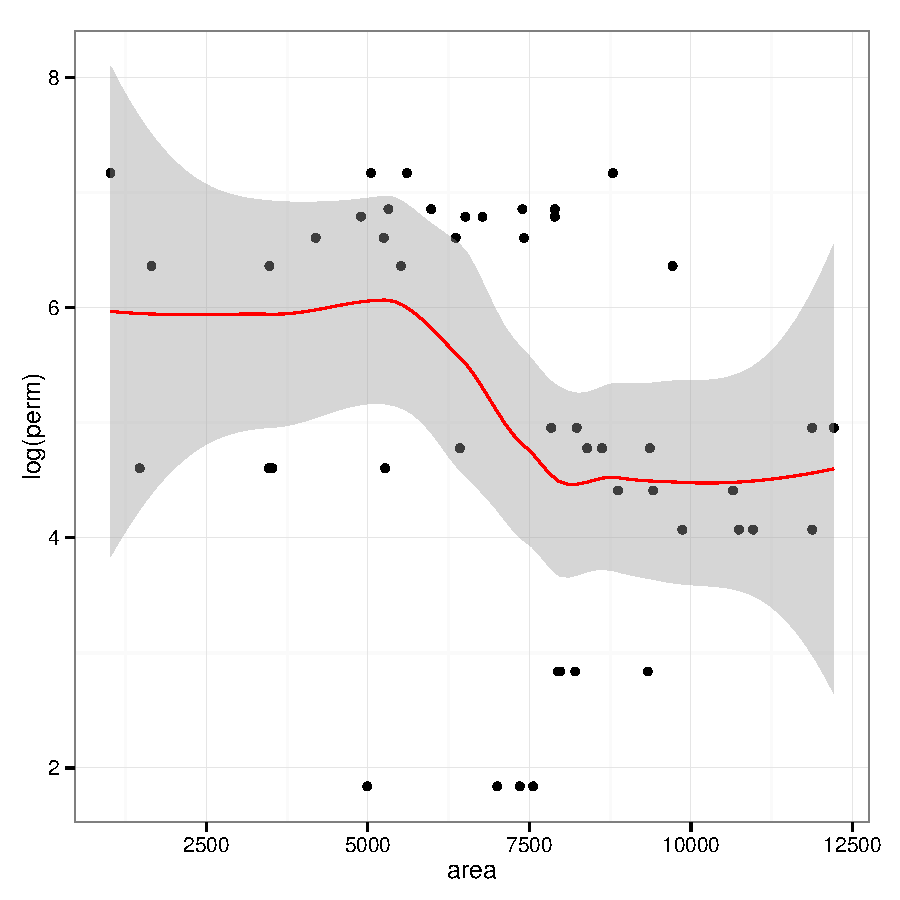
\includegraphics{Bericht_Sweave-002}

%Literaturverzeichnis
\newpage
\printbibliography 

\end{document}
